\documentclass[./../../paper.tex]{subfiles}
\graphicspath{{\subfix{./../../figures/}}}

\begin{document}


\label{sec:ssdld}
The \gls{damerau_levenshtein} function is a modified version of the Levenshstein distance\autocite{levenshtein_Binarycodescapable_1965}, which is a widely used to compute the edit-distance of two discrete sequences\autocites{apostolico_SequenceAlignmentMolecular_1998,Mitton20101}. The most important applications are within the \gls{NLP} discipline and the Biomedical Sciences. Within these areas, we often use the Levenshtein distance to compute the edit-distance between two words, two sentences or two DNA sequences. Note, that the elements of these sequences are often atomic symbols instead of multidimensional vectors. Generally, the distance accounts for inserts, deletions and substitutions of elements between the two serquences.
\citeauthor{damerau_techniquecomputerdetection_1964} modified the distance function to allow for transposition operations. For Process Mining, transpositions are important as one event can transition into two events that are processed in parallel and may have varying processing times.
% \attention{TODO: Check how a paper describes the reason for usage} 
In \autoref{fig:dl_example}, we schematically show two sequences and their distance.


\begin{figure}[htb]
    \centering
    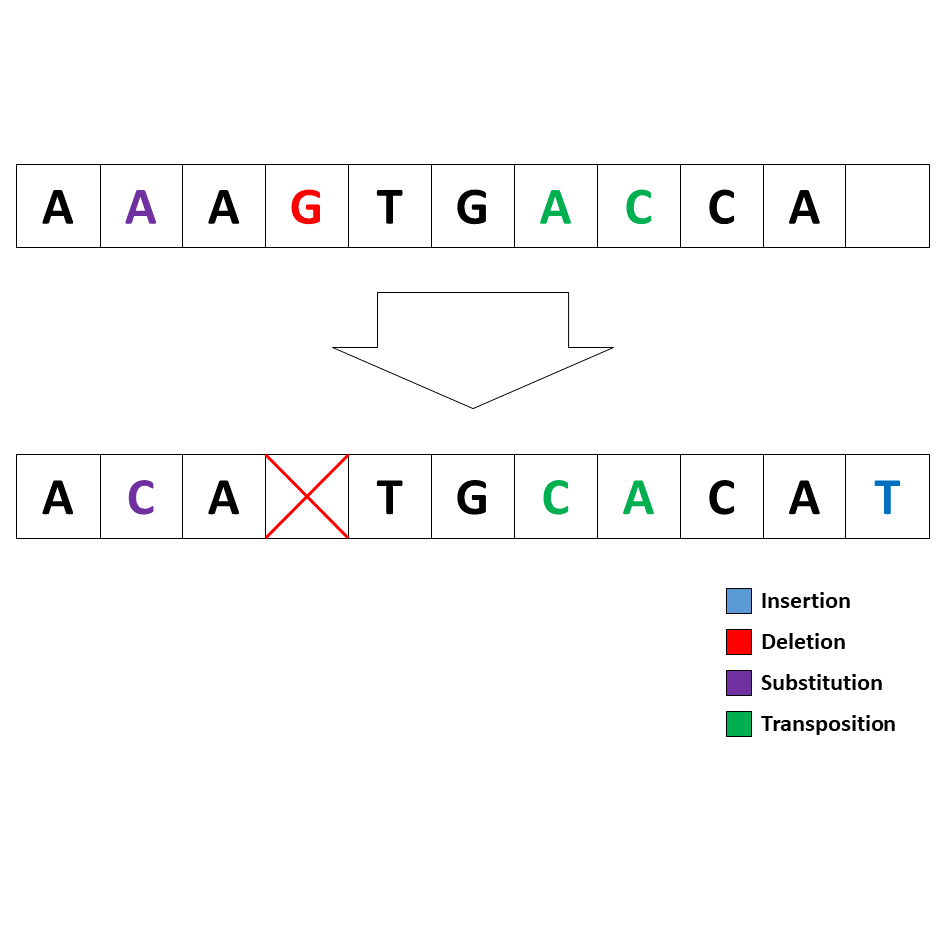
\includegraphics[width=0.75\textwidth]{figures/Graphics/Slide6.PNG}
    \caption{Shows two sequences. The edit distance is the sum of multiple operations. Blue shows an insert, red a deletion, purple a substitution and green a transposition. Therefore the edit distance is 4.}
    \label{fig:dl_example}
\end{figure}


\noindent In \autoref{eq:damerau_levenshstein} depicts the recursive formulation of the distance. The distance computes the costs of transforming the sequence $a$ to $b$, by computing the minimum of five seperate terms.  
% TODO: change a to e for consistency with model formulation
% TODO: Read on sequence alignment literature. Also add the readup to the literature review.
\begin{align}
    \label{eq:damerau_levenshstein}
    d_{a, b}(i, j) & =\min
    \begin{cases}
        \editDistance{i-1}{j  }+ 1 & \text { if } i>0                                            \\
        \editDistance{i  }{j-1}+ 1 & \text { if } j>0                                            \\
        \editDistance{i-1}{j-1}+ 1 & \text { if } i, j>0                                         \\
        \editDistance{i-2}{j-2}+ 1 & \text { if } i, j>1 \land a_{i}=b_{j-1} \land a_{i-1}=b_{j} \\
        0                                 & \text { if } i=j=0                                         
    \end{cases}        
\end{align}

\noindent The recursive form $d_{a, b}(i, j)$ for sequences $a$ and $b$ with respective elements $i$ and $j$ takes the minimum of each of each allowed edit operation. In particular, no change, deletion, insertion, substitution and transposition. For each operation, the algorithm adds an edit cost of 1. For Process Mining, it becomes necessary to modify the distance further. 

% TODO: Change a, b and c to x, y and z or e_1, e_2 and e_3
To illustrate the issue, we explore a couple of examples. Lets assume, we have two strings $s^1=aaba$ and $s^2=acba$. Using the Damerau-Levenshtein-Distance, the edit distance between both sequences is zero, as we can recognise one substitution at the second character in both strings. However, this representation is insufficient for process instances as they may also contain attibute values. Therefore, we characterise the sequences as process events in \autoref{eq:dlexample}. 

\begin{align}
    \label{eq:dlexample}
    s^1 &=\{a,a,b,a\} \\
    s^2 &=\{a,a^*,b,a\}\\
    s^3 &=\{a,c,b,a\}\\
    s^4 &=\{a,b,a\}
    &a,b,c \in \mathbb{R}^3\\
    a &= \begin{bmatrix}
        2\\
        1\\
        4\\
    \end{bmatrix}
    a^* = \begin{bmatrix}
        3\\
        3\\
        4\\
    \end{bmatrix}
    b = \begin{bmatrix}
        1\\
        1\\
        0\\
    \end{bmatrix}
    c = \begin{bmatrix}
        3\\
        1\\
        4\\
    \end{bmatrix}
\end{align}

\noindent If we do not consider attribute values, it becomes clear that $s^2$, $s^3$ and $s^4$ have an edit distance of 0, 1 and 1 to $s^1$. However, with attribute values $s^1$ and $s^2$ display clear differences. Similarly, $s^1$ and $s^3$ not only differ in terms of activity but also attribute value. Lastly, $s^1$ and $s^4$ are the same in attribute values, but one element still misses entirely. These examples show that we can neither disregard attribute values nor events, while computing the edit distance of two \glspl{instance}. 
We show this in \autoref{fig:image_with_dl}. 
In other words, we cannot simply assume a static cost of 1 for each edit operation. Instead, we have to define a cost function which takes attribute variables into account. In the following sections, we will establish distances which use a modified \gls{damerau_levenshtein} approach. Here, the cost of each edit-operation will be weighted with a distance function that considers the difference between event attributes. In simplified terms, we can say that $s^1$ and $s^2$ are identical, if we only consider the activity. However, taking attribute values into account, $s^1$ and $s^2$ actually differ on two accounts. 

% \begin{figure}[htb]
%     \centering
%     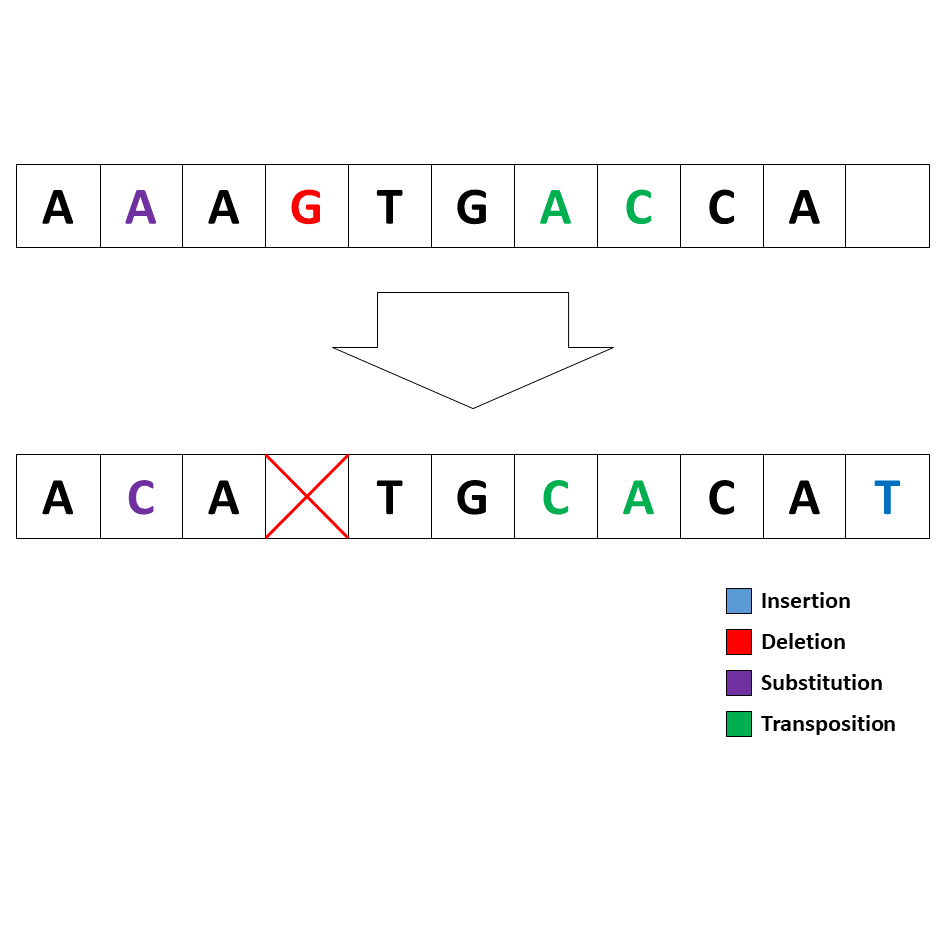
\includegraphics[width=0.99\textwidth]{figures/Graphics/Slide6.PNG}
%     \caption{This figure exemplifies the differeneces between the normal DL-distance and this one used.}
%     \label{fig:image_with_dl}
% \end{figure}

% \needsfigure{fig:image_with_dl}{This figure exemplifies the differeneces between the normal DL-distance and this one used.}

\noindent In order to reflect these differences in attribute values, we introduce a modified version of the \gls{damerau_levenshtein}, that not only reflects the difference between two process instances, but also the attribute values. We achieve this by introducing a cost function $\editCost$, which applies to a normed vector-space\footnotemark. Concretely, we formulate the modified \gls{damerau_levenshtein} as shown in \autoref{eq:modified_dl}. For the remainder, we will denote this edit-distance as \gls{SSDLD}.\footnotetext{A normed vector-space is a vector space, in which all vectors have the same dimensionality. For instance, if all vectors have three dimensions, we can call the vector-space \emph{normed}.}
% TODO: Introduce a with a dash above to compare activities instead of the vector
% Make zero thicker to indicate a null vector
\begin{align}
    \label{eq:modified_dl}
    d_{a, b}(i, j) & =\min
    \begin{cases}
        \editDistance{i-1}{j  }+\editCostFunctionNoA & \text { if } i>0                                            \\
        \editDistance{i  }{j-1}+\editCostFunctionNoB & \text { if } j>0                                            \\
        \editDistance{i-1}{j-1}+\editCostFunctionBoth & \text { if } i, j>0   \\ & \text { \& } \overline{a}_i=\overline{b}_j                                       \\
        \editDistance{i-1}{j-1}+ \editCostFunctionNoB +\editCostFunctionNoA  & \text { if } i, j>0  \\ & \text { \& } \overline{a}_i \neq \overline{b}_j                                       \\
        \editDistance{i-2}{j-2}+\editCostFunction{a_i}{b_{j-1}} + \editCostFunction{a_{i-1}}{b_j} & \text { if } i, j>1 \\ 
        & \text { \& } \overline{a}_i=\overline{b}_{j-1} \\ 
        & \text { \& } \overline{a}_{i-1}=\overline{b}_j \\
        0                                 & \text { \& } i=j=0                                          
    \end{cases} 
\end{align}

\noindent Here, $d_{a, b}(i, j)$ is the recursive form of the Damerau-Levenshtein-Distance. $a$ and $b$ are sequences and $i$ and $j$ specific elements of the sequence. $cost(a,b)$ is a cost function which takes the attribute values of $a$ and $b$ into account. 
The first two terms correspond to a deletion and an insertion from $a$ to $b$. The idea is to compute the maximal cost for that the wrongfully deleted or inserted event. 
The third term adds the difference between two events with identical activities $\overline{a}_i$ and $\overline{b}_j$. As mentioned earlier, two events that refer to the same activity can still be different due to event attributes. The distance between the event attributes determines \emph{how} different these events are. 
The fourth term handles the substitution of two events. Here, we compute the substitution cost as the sum of an insertion and a deletion. 
The fifth term computes the cost after transposing both events. This cost is similar to term 3 only that we now consider the differences between both events after they were aligned. The last term relates to the stopping criterion of the recursive formulation of the \gls{damerau_levenshtein}.  


\end{document}